% Provenance (never printed): see sources/outline_sources.md (Year 2: partial melting of the
% mantle; solidus and geotherm; decompression, hydration and heating; degree of melting;
% binary and ternary phase diagrams applied to rocks).
% Curves from figdata/bachelor-2/melting.py (Bowen 1915 diopside-anorthite, Bowen and
% Andersen 1914 forsterite-silica, Katz et al. 2003 melting of peridotite); exercise and
% problem values in the Book 4 scratch calculator calc/ch07.py.
\chapter{De mantel smelten}\label{ch:b2:mantle-melting}

De mantel is vast. Seismische schuifgolven doorkruisen hem van boven tot onder, en het
\omterm{def:b2:mantle-melting:peridotites}{peridotiet} dat eruit naar boven komt, is een kristallijn gesteente. Toch levert hij alleen al langs de
oceanische ruggen elk jaar zo'n twintig kubieke kilometer nieuwe oceanische korst,
waarvan elke kubieke meter uit een smelt is gemaakt. De paradox verdwijnt zodra men weet
dat de mantel niet smelt omdat hij wordt verhit: hij smelt omdat de
druk erop daalt, of omdat er water aan wordt toegevoegd. Onder een rug
stijgt de mantel op, daalt zijn druk sneller dan zijn temperatuur, en overschrijdt hij zijn
smeltkromme; boven een zinkende plaat verlaagt water dat uit de plaat vrijkomt die
kromme onder de mantelwig. In beide gevallen smelt slechts een kleine fractie van het gesteente,
en die fractie, gescheiden van haar residu, wordt het basalt van de
oceaanbodem en van de vulkanische bogen. Dit hoofdstuk beschrijft eerst het
mantelgesteente en de fasediagrammen die vertellen hoe zulke gesteenten smelten, en volgt daarna de
mantel omhoog onder een rug tot aan de dikte van de korst die hij maakt.
% ledger: white:crust (Book 3), data:pb2002 (Book 3), katz03:solidus

\begin{recall}
\textbf{Uit het scheikundeboek van het tweede jaar universiteit}: binaire fasediagrammen, de
solidus en de liquidus, het eutectisch punt, congruent smelten, vaste oplossingen
en de hefboomregel, volgens welke de verhoudingen van twee naast elkaar bestaande fasen
omgekeerd evenredig zijn met hun afstanden tot de totale samenstelling.
\textbf{Uit de natuurkundeboeken}: de soortelijke warmte, de latente warmte, de entropie
en de tweede hoofdwet, volgens welke een reversibel adiabatisch proces de entropie behoudt.
\textbf{Uit Boek~3}: de belangrijkste gesteentevormende mineralen, olivijn,
pyroxenen, granaat en spinel, hun vaste oplossingen en het Mg-getal; de
manteladiabaat, $\mathrm dT/\mathrm dz = \alpha gT/c_p$; de oceanische korst,
\qty[uncertainty-mode=separate]{7.1 \pm 0.8}{km} dik ver van hotspots en
ongeveer \qty{20}{km} boven de kern van een pluim; subducerende platen en het water dat ze
meevoeren. \textbf{Uit \cref{ch:b2:elements-in-the-earth}}: \omterm{def:b2:elements-in-the-earth:morb-oib}{basalt van mid-oceanische ruggen}
(MORB), verdelingscoëfficiënten en \omterm{def:b2:elements-in-the-earth:partition}{incompatibele elementen}.
\end{recall}

\section{Het mantelgesteente}\label{sec:b2:mantle-melting:rock}

Mantelgesteente bereikt het oppervlak als fragmenten die door \omterm{def:b2:magma-emplacement:magma}{magma's} worden meegevoerd, de
xenolieten, en als de basis van schollen oceanische lithosfeer die op de
continenten zijn geschoven, de ofiolieten. Bijna alles ervan is \omterm{def:b2:mantle-melting:peridotites}{peridotiet}.
% ledger: geo:peridotite (Book 2), tulane:ocean-basins (Book 2)

\begin{definition}[Peridotiet en zijn soorten]\label{def:b2:mantle-melting:peridotites}
Een \emph{peridotiet}\index{peridotiet} is een grofkorrelig ultramafisch gesteente
met meer dan \qty{40}{\percent} olivijn, waarbij de rest uit pyroxenen en een
beetje van een aluminiumhoudend mineraal (spinel of granaat) bestaat. Een
\emph{duniet}\index{duniet} bevat meer dan \qty{90}{\percent} olivijn. Daaronder
bevat een \emph{lherzoliet}\index{lherzoliet} zowel orthopyroxeen als
clinopyroxeen; een \emph{harzburgiet}\index{harzburgiet} bevat orthopyroxeen maar
bijna geen clinopyroxeen; een wehrliet bevat clinopyroxeen maar bijna geen
orthopyroxeen. Gesteenten met minder dan \qty{40}{\percent} olivijn zijn pyroxenieten.
\end{definition}
% ledger: bgs:ultramafic

De indeling wordt afgelezen op een driehoek met als hoekpunten olivijn,
orthopyroxeen en clinopyroxeen (de figuur hieronder): elk punt staat voor een gesteente,
en zijn afstanden tot de drie zijden geven de verhoudingen van de drie
mineralen. Een modelsamenstelling van de verarmde bovenmantel die onder
de ruggen smelt, heeft \qty{57}{\percent} olivijn,
\qty{28}{\percent} orthopyroxeen, \qty{13}{\percent} clinopyroxeen en
\qty{2}{\percent} spinel: een \omterm{def:b2:mantle-melting:peridotites}{lherzoliet}.
% ledger: liang21:dmm-mode

\begin{omfigure}
\centering
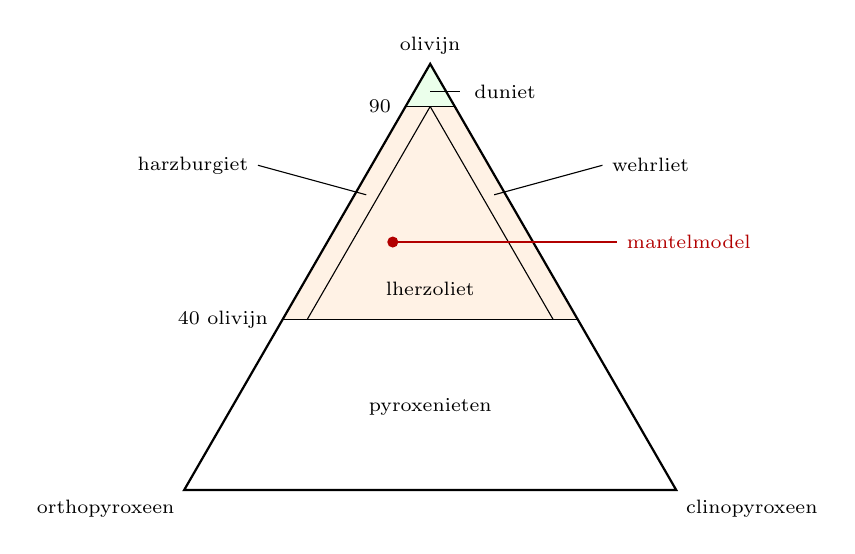
\begin{tikzpicture}[x=1.25cm, y=1.25cm, font=\scriptsize]
\coordinate (O) at (2.5,4.330); \coordinate (P) at (0,0); \coordinate (C) at (5,0);
\fill[green!8] (2.25,3.897) -- (2.75,3.897) -- (O) -- cycle;
\fill[orange!10] (1,1.732) -- (2.25,3.897) -- (2.75,3.897) -- (4,1.732) -- cycle;
\draw[thick] (O) -- (P) -- (C) -- cycle;
\draw (2.25,3.897) -- (2.75,3.897);
\draw (1,1.732) -- (4,1.732);
\draw (2.5,3.897) -- (1.25,1.732);
\draw (2.5,3.897) -- (3.75,1.732);
\node[anchor=south] at (O) {olivijn};
\node[anchor=north east] at (P) {orthopyroxeen};
\node[anchor=north west] at (C) {clinopyroxeen};
\node[anchor=west] at (2.85,4.05) {duniet};
\draw (2.5,4.05) -- (2.8,4.05);
\node at (2.5,2.05) {lherzoliet};
\draw (1.85,3.0) -- (0.75,3.3) node[anchor=east] {harzburgiet};
\draw (3.15,3.0) -- (4.25,3.3) node[anchor=west] {wehrliet};
\node at (2.5,0.85) {pyroxenieten};
\node[anchor=east] at (0.95,1.732) {\qty{40}{\percent} olivijn};
\node[anchor=east] at (2.2,3.897) {\qty{90}{\percent}};
\fill[red!70!black] (2.12,2.52) circle (2pt);
\draw[red!70!black] (2.12,2.52) -- (4.4,2.52) node[anchor=west] {mantelmodel};
\end{tikzpicture}
\par\smallskip{\small Indeling van de \omterm{def:b2:mantle-melting:peridotites}{peridotieten} en pyroxenieten naar hun
verhoudingen van olivijn, orthopyroxeen en clinopyroxeen (naar het schema van de British
Geological Survey). De smalle stroken langs de twee bovenste zijden bevatten de
gesteenten met bijna geen clinopyroxeen (\omterm{def:b2:mantle-melting:peridotites}{harzburgiet}) of geen orthopyroxeen (wehrliet).
De rode stip is de model-bovenmantel onder de ruggen (57, 28 en
\qty{13}{\percent}, hergenormaliseerd zonder zijn \qty{2}{\percent} spinel).}
\end{omfigure}
% ledger: bgs:ultramafic, liang21:dmm-mode

De drie \omterm{def:b2:mantle-melting:peridotites}{peridotieten} zijn geen drie onafhankelijke gesteentesoorten: het zijn stadia van
één proces. Clinopyroxeen en het aluminiumhoudende mineraal raken als eerste op wanneer
\omterm{def:b2:mantle-melting:peridotites}{peridotiet} smelt (\cref{sec:b2:mantle-melting:decompression}), dus een \omterm{def:b2:mantle-melting:peridotites}{lherzoliet}
die een smelt heeft verloren, wordt er armer aan; na genoeg smelten is het een
\omterm{def:b2:mantle-melting:peridotites}{harzburgiet}, en een gesteente dat bijna al zijn pyroxeen heeft verloren, is een \omterm{def:b2:mantle-melting:peridotites}{duniet}.
% ledger: katz03:melting

\begin{definition}[Fertiele en residuele mantel]\label{def:b2:mantle-melting:fertility}
Een \emph{fertiele mantel}\index{fertiele mantel} is een \omterm{def:b2:mantle-melting:peridotites}{peridotiet}, meestal een
\omterm{def:b2:mantle-melting:peridotites}{lherzoliet}, dat nog het clinopyroxeen en het aluminiumhoudende mineraal bevat waaruit
basalt wordt gemaakt. Een \emph{residuele mantel}\index{residuele mantel} is het
\omterm{def:b2:mantle-melting:peridotites}{peridotiet} dat achterblijft nadat er een smelt aan is onttrokken: armer aan
clinopyroxeen, aluminium, calcium en de \omterm{def:b2:elements-in-the-earth:partition}{incompatibele elementen}, rijker aan
olivijn en met een hoger Mg-getal.
\end{definition}

De isotopisch \omterm{def:b2:isotope-geochemistry:reservoirs}{verarmde mantel} van \cref{ch:b2:isotope-geochemistry} is een reservoir,
gedefinieerd door zijn verhoudingen; een \omterm{def:b2:mantle-melting:fertility}{residuele mantel} is een gesteente, gedefinieerd door wat het heeft verloren.
De twee hangen samen, want de \omterm{def:b2:isotope-geochemistry:reservoirs}{verarmde mantel} is verarmd omdat er lang geleden smelt aan werd
onttrokken, maar het ene wordt in een massaspectrometer gelezen en het andere
onder de microscoop.

\section{Fasediagrammen van gesteenten}\label{sec:b2:mantle-melting:diagrams}

Een gesteente is een mengsel van mineralen, en het smelt over een temperatuurbereik, niet in
één punt. De diagrammen die dit beschrijven, werden eerst gemeten aan mengsels van
zuivere synthetische mineralen, door een kleine lading op een bekende temperatuur te houden tot ze
in evenwicht was, haar af te schrikken, en onder de microscoop te zoeken naar glas,
dat vloeibaar was geweest, en kristallen.

\subsection*{Een binair eutecticum: diopsied en anorthiet}

Een basalt bestaat in wezen uit een calciumrijk plagioklaas en een clinopyroxeen, en
Bowen koos zuiver anorthiet en diopsied als zijn eenvoudigste model. Gemengd en verhit,
vormen ze een gewoon eutectisch
systeem (de figuur hieronder): diopsied smelt bij \qty{1391.5}{\celsius} en anorthiet
bij \qty{1550}{\celsius}, maar een mengsel van \qty{58}{\percent} diopsied en
\qty{42}{\percent} anorthiet in massa smelt volledig bij \qty{1270}{\celsius}.
% ledger: bowen15:di-an

\begin{omfigure}
\centering
\begin{tikzpicture}
\begin{axis}[omrecord, width=0.78\linewidth, height=6cm,
  xmin=0, xmax=100, ymin=1200, ymax=1600,
  xlabel={anorthiet (\unit{\percent} in massa)}, ylabel={temperatuur (\unit{\celsius})},
  y tick label style={/pgf/number format/1000 sep={}},
  tick label style={font=\scriptsize}, label style={font=\small}]
\addplot[very thick, black] table[x=x_an, y=T] {figdata/out/bachelor-2-melting-di-an-liq.dat};
\addplot[only marks, mark=*, mark size=1.6pt, blue!70!black] table[x=x_an, y=T] {figdata/out/bachelor-2-melting-di-an-data.dat};
\draw[thick] (axis cs:0,1270) -- (axis cs:100,1270);
\draw[densely dotted, red!70!black, thick] (axis cs:20,1590) -- (axis cs:20,1270);
\draw[->, red!70!black, thick] (axis cs:20,1350) -- (axis cs:41,1272);
\fill[red!70!black] (axis cs:20,1350) circle (1.6pt);
\node[font=\scriptsize] at (axis cs:55,1500) {smelt};
\node[font=\scriptsize, align=center] at (axis cs:10,1300) {diopsied\\+ smelt};
\node[font=\scriptsize, align=center] at (axis cs:72,1360) {anorthiet + smelt};
\node[font=\scriptsize] at (axis cs:68,1235) {diopsied + anorthiet};
\node[font=\scriptsize, anchor=north east] at (axis cs:41,1267) {E, \qty{1270}{\celsius}};
\node[font=\scriptsize, anchor=west, red!70!black] at (axis cs:21,1360) {eerste diopsied};
\end{axis}
\end{tikzpicture}
\par\smallskip{\small Het systeem diopsied--anorthiet bij atmosferische druk, uit
de afschrikexperimenten van Bowen (1915): liquidustemperaturen (stippen, midden van
de afschrikintervallen) en het eutecticum E. In het rood de afkoeling van een smelt van
\qty{20}{\percent} anorthiet: diopsied kristalliseert vanaf \qty{1350}{\celsius}, de
smelt daalt langs de liquidus naar E, en de rest kristalliseert daar als een mengsel van
beide mineralen.}
\end{omfigure}
% ledger: bowen15:di-an

Van boven gelezen geeft het diagram de kristallisatievolgorde. Een smelt van
\qty{20}{\percent} anorthiet begint diopsied te kristalliseren bij
\qty{1350}{\celsius}; de smelt verliest diopsied, wordt rijker aan anorthiet en
daalt langs de liquidus tot hij het eutecticum bereikt, waar anorthiet zich bij
diopsied voegt en de temperatuur op \qty{1270}{\celsius} blijft tot alle smelt
verdwenen is. Van onderen gelezen geeft het hoe het gesteente smelt: wat de verhoudingen van
de twee mineralen ook zijn, de eerste smelt verschijnt bij \qty{1270}{\celsius} en heeft de
eutectische samenstelling. Dat is de eerste les voor de mantel. De eerste smelt van een
gesteente heeft niet de samenstelling van het gesteente: ze heeft de samenstelling die wordt vastgelegd door de
mineralen waaruit ze smelt, en ze verschijnt bij een temperatuur ver onder de
smeltpunten van al die mineralen.

\subsection*{Incongruent smelten: forsteriet en silica}

Sommige mineralen smelten niet tot een smelt met hun eigen samenstelling.

\begin{definition}[Incongruent smelten, peritectisch punt]\label{def:b2:mantle-melting:peritectic}
Een mineraal vertoont \emph{incongruent smelten}\index{incongruent smelten} wanneer het bij
verhitting uiteenvalt in een andere vaste stof en een smelt met een andere
samenstelling, in plaats van te smelten tot een smelt met zijn eigen samenstelling. Op een binair
fasediagram is het punt waar die smelt naast beide vaste stoffen bestaat een
\emph{peritectisch punt}\index{peritectisch punt}: anders dan een eutecticum ligt het niet
tussen de samenstellingen van de twee vaste stoffen.
\end{definition}

Enstatiet, het magnesiumrijke orthopyroxeen \ce{MgSiO3}, smelt incongruent. Bij
atmosferische druk valt het bij \qty{1557}{\celsius} uiteen in forsteriet,
\ce{Mg2SiO4}, en een smelt die iets rijker aan silica is dan het enstatiet zelf; pas bij
\qty{1577}{\celsius} is al het forsteriet opgelost (de figuur hieronder). Bowen
en Andersen vonden in 1914 dat het uiteenvallen \qty{5.5}{\percent}
forsteriet en \qty{94.5}{\percent} smelt geeft, zoals de hefboomregel voorspelt uit
de drie samenstellingen (\cref{exo:b2:mantle-melting:6}). Verder naar silica toe smelten enstatiet en
cristobaliet samen in een eutecticum, \qty{1543}{\celsius}.
% ledger: bowen14:mgo-sio2

\begin{omfigure}
\centering
\begin{tikzpicture}
\begin{axis}[omrecord, width=0.78\linewidth, height=6cm,
  xmin=40, xmax=66, ymin=1450, ymax=1950,
  xlabel={\ce{SiO2} (\unit{\percent} in massa)}, ylabel={temperatuur (\unit{\celsius})},
  y tick label style={/pgf/number format/1000 sep={}},
  tick label style={font=\scriptsize}, label style={font=\small}]
\addplot[very thick, black] table[x=x_sio2, y=T] {figdata/out/bachelor-2-melting-fo-sio2-liq.dat};
\addplot[very thick, black, dashed] table[x=x_sio2, y=T] {figdata/out/bachelor-2-melting-fo-sio2-fo.dat};
\draw[thick] (axis cs:42.71,1450) -- (axis cs:42.71,1890);
\draw[thick] (axis cs:42.71,1557) -- (axis cs:60.86,1557);
\draw[thick] (axis cs:59.85,1450) -- (axis cs:59.85,1557);
\draw[thick] (axis cs:59.85,1543) -- (axis cs:66,1543);
\fill (axis cs:60.86,1557) circle (1.6pt);
\fill (axis cs:64.87,1543) circle (1.6pt);
\fill (axis cs:42.71,1890) circle (1.6pt);
\node[font=\scriptsize, anchor=south west] at (axis cs:42.9,1890) {forsteriet smelt, \qty{1890}{\celsius}};
\node[font=\scriptsize] at (axis cs:56,1800) {smelt};
\node[font=\scriptsize] at (axis cs:48,1680) {forsteriet + smelt};
\node[font=\scriptsize] at (axis cs:51,1500) {forsteriet + enstatiet};
\node[font=\scriptsize, align=center] at (axis cs:63,1495) {enstatiet +\\cristobaliet};
\node[font=\scriptsize, anchor=south] at (axis cs:61.3,1560) {P};
\node[font=\scriptsize, anchor=south] at (axis cs:64.87,1546) {E};
\node[font=\scriptsize, anchor=north, rotate=90] at (axis cs:42.71,1650) {\ce{Mg2SiO4}};
\node[font=\scriptsize, anchor=south, rotate=90] at (axis cs:59.85,1510) {\ce{MgSiO3}};
\end{axis}
\end{tikzpicture}
\par\smallskip{\small Deel van het systeem \ce{MgO}--\ce{SiO2} bij atmosferische
druk, naar Bowen en Andersen (1914). Enstatiet (\ce{MgSiO3}) smelt
incongruent in het \omterm{def:b2:mantle-melting:peritectic}{peritectisch punt} P, \qty{1557}{\celsius}, tot forsteriet en een
smelt van \qty{60.9}{\percent} \ce{SiO2}; E is het eutecticum enstatiet--cristobaliet,
\qty{1543}{\celsius}. De liquidus van forsteriet is alleen dicht bij
enstatiet gemeten: het gestreepte deel is recht doorgetrokken tot het smeltpunt van forsteriet.}
\end{omfigure}
% ledger: bowen14:mgo-sio2

Het \omterm{def:b2:mantle-melting:peritectic}{peritectisch punt} is de tweede les voor de mantel. Wanneer een \omterm{def:b2:mantle-melting:peridotites}{peridotiet} smelt, lost zijn
orthopyroxeen niet gewoon op: het geeft olivijn aan het residu en silica
aan de smelt. De smelt is daarom rijker aan silica dan de pyroxenen, en het
residu rijker aan olivijn dan het gesteente: de weg van \omterm{def:b2:mantle-melting:peridotites}{lherzoliet} naar \omterm{def:b2:mantle-melting:peridotites}{harzburgiet}
en \omterm{def:b2:mantle-melting:peridotites}{duniet}.

\subsection*{Drie componenten: het ternaire diagram}

Echte gesteenten hebben meer dan twee mineralen. Met drie vraagt de samenstelling een
driehoek, en wordt de temperatuur een derde dimensie.

\begin{definition}[Ternair fasediagram, cotectische lijn, ternair eutecticum]\label{def:b2:mantle-melting:ternary}
Een \emph{ternair fasediagram}\index{ternair fasediagram} stelt de
evenwichten van een systeem van drie componenten bij een gegeven druk voor: elk punt van een
driehoek staat voor een samenstelling, de hoekpunten voor de zuivere componenten, en het
liquidusoppervlak wordt getekend als temperatuurcontouren of als de velden van de
mineralen die als eerste kristalliseren. Een \emph{cotectische lijn}\index{cotectische lijn} is
de lijn waarlangs de smelt tegelijk verzadigd is in twee mineralen en
beide kristalliseert terwijl hij afkoelt. De cotectische lijnen dalen af van de binaire
eutectica op de zijden van de driehoek en ontmoeten elkaar in het \emph{ternaire
eutecticum}\index{ternair eutecticum}, de laagste temperatuur waarbij smelt bestaat,
waar de drie mineralen samen kristalliseren.
\end{definition}

\begin{method}[Een kristallisatieweg aflezen op een ternair diagram]\label{met:b2:mantle-melting:ternary}
Zoek de totale samenstelling $X$ in de driehoek en het veld waarin ze ligt:
het mineraal van dat veld kristalliseert als eerste. Zolang alleen dat mineraal kristalliseert,
beweegt de smelt in een rechte lijn recht weg van het hoekpunt van het mineraal,
door $X$, omdat het verwijderen van een zuivere component alleen het aandeel ervan verandert; volgens de
hefboomregel is de massafractie kristallen de afstand van $X$ tot de smelt
gedeeld door de afstand van het hoekpunt tot de smelt. Wanneer de smelt een
\omterm{def:b2:mantle-melting:ternary}{cotectische lijn} bereikt, voegt het tweede mineraal zich erbij en volgt de smelt de \omterm{def:b2:mantle-melting:ternary}{cotectische lijn}
omlaag naar het \omterm{def:b2:mantle-melting:ternary}{ternaire eutecticum}, waar de laatste smelt kristalliseert. Een component
die in geen van de kristallen terechtkomt, blijft in de smelt, dus zijn concentratie geeft
de fractie resterende smelt: $f_{\text{smelt}} = c_X/c_{\text{smelt}}$.
\end{method}

\begin{omfigure}
\centering
\begin{tikzpicture}[x=1cm, y=1cm, font=\scriptsize]
\coordinate (A) at (3,5.196); \coordinate (B) at (0,0); \coordinate (C) at (6,0);
\coordinate (eAB) at (1.2,2.078); \coordinate (eAC) at (4.65,2.338);
\coordinate (eBC) at (3.9,0); \coordinate (E) at (3.45,1.299);
\coordinate (X) at (3.0,3.118); \coordinate (L) at (3.0,1.455);
\fill[green!8] (A) -- (eAB) -- (E) -- (eAC) -- cycle;
\fill[orange!10] (B) -- (eAB) -- (E) -- (eBC) -- cycle;
\fill[blue!7] (C) -- (eAC) -- (E) -- (eBC) -- cycle;
\draw[thick] (A) -- (B) -- (C) -- cycle;
\draw[very thick, -{Stealth[length=4pt]}] (eAB) -- ($(eAB)!0.55!(E)$);
\draw[very thick] ($(eAB)!0.5!(E)$) -- (E);
\draw[very thick, -{Stealth[length=4pt]}] (eAC) -- ($(eAC)!0.55!(E)$);
\draw[very thick] ($(eAC)!0.5!(E)$) -- (E);
\draw[very thick, -{Stealth[length=4pt]}] (eBC) -- ($(eBC)!0.55!(E)$);
\draw[very thick] ($(eBC)!0.5!(E)$) -- (E);
\draw[red!70!black, thick, dashed] (A) -- (X);
\draw[red!70!black, very thick, -{Stealth[length=4pt]}] (X) -- (L);
\draw[red!70!black, very thick, -{Stealth[length=4pt]}] (L) -- ($(L)!0.85!(E)$);
\fill[red!70!black] (X) circle (2pt); \fill[red!70!black] (L) circle (1.6pt);
\fill (E) circle (2pt);
\node[anchor=south] at (A) {A}; \node[anchor=north east] at (B) {B};
\node[anchor=north west] at (C) {C};
\node[anchor=west, red!70!black] at (3.1,3.2) {$X$};
\node[anchor=north east, red!70!black] at (2.95,1.42) {$L_1$};
\node[anchor=north west] at (3.5,1.25) {E};
\node[anchor=east] at (eAB) {$e_{AB}$}; \node[anchor=west] at (eAC) {$e_{AC}$};
\node[anchor=north] at (eBC) {$e_{BC}$};
\node at (2.35,2.75) {veld A}; \node at (1.55,0.7) {veld B}; \node at (4.9,0.7) {veld C};
\end{tikzpicture}
\par\smallskip{\small Een ternair eutectisch systeem (schematisch). Elk veld bevat
de smelten waaruit zijn mineraal als eerste kristalliseert; de \omterm{def:b2:mantle-melting:ternary}{cotectische lijnen} (pijlen
naar dalende temperatuur) lopen van de binaire eutectica $e$ naar het \omterm{def:b2:mantle-melting:ternary}{ternaire
eutecticum} E. Een smelt $X$ in het veld A kristalliseert A, en beweegt weg van het hoekpunt
A tot hij de \omterm{def:b2:mantle-melting:ternary}{cotectische lijn} A--B ontmoet in $L_1$; A en B kristalliseren dan
samen tot E, waar C zich bij hen voegt (\cref{exo:b2:mantle-melting:11}).}
\end{omfigure}

Systemen van drie gesteentevormende mineralen worden op dezelfde manier gelezen. De regels die bepalen hoeveel fasen naast elkaar kunnen bestaan,
en de vrije-energieoppervlakken waaruit zulke diagrammen worden berekend, horen bij
Boek~5 van deze reeks.

\section{Solidus, adiabaat en drie manieren om te smelten}\label{sec:b2:mantle-melting:solidus}

Mantelperidotiet heeft een solidus, de temperatuur waarbij zijn eerste smelt verschijnt,
en een liquidus ver daarboven. Beide stijgen met de druk. Experimenten met natuurlijke
\omterm{def:b2:mantle-melting:peridotites}{peridotieten}, verzameld en gefit door Katz, Spiegelman en Langmuir in 2003, geven
voor de droge solidus
\[
  T_{\mathrm{s}}(P) = 1085.7 + 132.9\,P - 5.1\,P^2
\]
(in graden Celsius, $P$ in gigapascal): \qty{1086}{\celsius} aan het oppervlak,
\qty{1331}{\celsius} bij \qty{2}{GPa}. Op dezelfde diepten is de mantel heter of
kouder dan dit, afhankelijk van waar hij ligt, en om mantels te vergelijken neemt men het
effect van de diepte weg.
% ledger: katz03:solidus

\begin{definition}[Potentiële manteltemperatuur]\label{def:b2:mantle-melting:tp}
De \emph{potentiële manteltemperatuur}\index{potentiële manteltemperatuur} $T_p$
is de temperatuur die een pakket convecterende mantel zou hebben als het langs de manteladiabaat
naar het oppervlak werd gebracht, zonder warmte uit te wisselen en
zonder te smelten.
\end{definition}

Langs de adiabaat geldt $\mathrm dT/\mathrm dP = \alpha T/(\rho c_p)$, de vorm in
druk van de hierboven herhaalde gradiënt $\alpha gT/c_p$, want $\mathrm dP = \rho
g\,\mathrm dz$. Met $\alpha = \qty{4e-5}{K^{-1}}$, $\rho = \qty{3300}{kg/m^3}$
en $c_p = \qty{1000}{J/(kg.K)}$ is dat ongeveer \qty{20}{K} per gigapascal, waarbij een
gigapascal overeenkomt met \qty{30.9}{km} mantel (\cref{exo:b2:mantle-melting:3}). Boek~3 gaf
de mantel een potentiële temperatuur van ongeveer \qty{1350}{\celsius} uit de
mineraalfysica; petrologische schattingen voor de mantel onder ruggen lopen van 1280 tot
\qty{1400}{\celsius}.
% ledger: katz03:thermo, katsura:adiabat (Book 3), herzberg:tp (Book 3)

\begin{proposition}[Begin van decompressiesmelten]\label{prop:b2:mantle-melting:onset}
Mantel met potentiële temperatuur $T_p$ die opstijgt langs de adiabaat $T = T_p + GP$ ($G$
constant), begint te smelten bij de druk $P_0$ waar de adiabaat de
solidus $T_{\mathrm s}(P) = a_1 + a_2P + a_3P^2$ snijdt, de kleinste wortel van
\[
  -a_3P^2 + (G - a_2)P + (T_p - a_1) = 0 .
\]
Een mantel die $\Delta T_p$ heter is, begint dieper te smelten, met $\Delta P_0 \approx
\Delta T_p/(T_{\mathrm s}'(P_0) - G)$.
\end{proposition}

\begin{proof}
Op diepte is de adiabaat kouder dan de solidus, omdat de solidus
steiler stijgt ($T_{\mathrm
s}' \approx \qty{110}{K/GPa}$ tegen $G \approx 20$). De twee krommen snijden elkaar waar
$T_p + GP = a_1 + a_2P + a_3P^2$, wat tot de vierkantsvergelijking herschikt. Differentiëren van
$T_p + GP_0 = T_{\mathrm s}(P_0)$ geeft $\mathrm dT_p = (T_{\mathrm s}'(P_0) -
G)\,\mathrm dP_0$.
\end{proof}

Voor $T_p = \qty{1350}{\celsius}$ ligt het begin bij \qty{2.66}{GPa}, ongeveer
\qty{82}{km} diep, bij \qty{1403}{\celsius}; elke \qty{10}{\celsius} potentiële
temperatuur verschuift het met ongeveer \qty{0.12}{GPa}, of \qty{3.6}{km}. De figuur hieronder
toont de solidus en de adiabaten.

\begin{omfigure}
\centering
\begin{tikzpicture}
\begin{axis}[omrecord, width=0.8\linewidth, height=7cm,
  xmin=850, xmax=2000, ymin=0, ymax=6, y dir=reverse,
  xlabel={temperatuur (\unit{\celsius})}, ylabel={druk (\unit{GPa})},
  x tick label style={/pgf/number format/1000 sep={}},
  axis y line*=left,
  legend style={font=\scriptsize, at={(0.5,-0.2)}, anchor=north, legend columns=3},
  tick label style={font=\scriptsize}, label style={font=\small}]
\addplot[very thick, black] table[x=Ts, y=P_GPa] {figdata/out/bachelor-2-melting-pt.dat};
\addlegendentry{droge solidus}
\addplot[thick, black, densely dotted] table[x=Tl, y=P_GPa] {figdata/out/bachelor-2-melting-pt.dat};
\addlegendentry{liquidus van lherzoliet}
\addplot[thick, black, dashed] table[x=Tq, y=P_GPa] {figdata/out/bachelor-2-melting-pt.dat};
\addlegendentry{liquidus}
\addplot[thick, blue!70!black, dashdotted] table[x=wetsat, y=P_GPa] {figdata/out/bachelor-2-melting-pt.dat};
\addlegendentry{watergezadigde solidus}
\addplot[thick, red!70!black] table[x=ad1350, y=P_GPa] {figdata/out/bachelor-2-melting-pt.dat};
\addlegendentry{adiabaten, $T_p$ = 1300, 1350, \qty{1450}{\celsius}}
\addplot[thin, red!70!black] table[x=ad1300, y=P_GPa] {figdata/out/bachelor-2-melting-pt.dat};
\addplot[thin, red!70!black] table[x=ad1450, y=P_GPa] {figdata/out/bachelor-2-melting-pt.dat};
\addplot[only marks, mark=*, mark size=2pt, red!70!black] table[x=T0, y=P0] {figdata/out/bachelor-2-melting-onset.dat};
\end{axis}
\begin{axis}[width=0.8\linewidth, height=7cm, xmin=850, xmax=2000,
  ymin=0, ymax=185.34, y dir=reverse, axis y line*=right, axis x line=none,
  ylabel={diepte (\unit{km})}, tick label style={font=\scriptsize}, label style={font=\small}]
\end{axis}
\end{tikzpicture}
\par\smallskip{\small Smeltkrommen van droog \omterm{def:b2:mantle-melting:peridotites}{peridotiet} en de watergezadigde
solidus volgens de parametrisering van Katz en anderen (2003), met doorgetrokken adiabaten
voor drie potentiële temperaturen; de stippen markeren het begin van het smelten,
\qty{2.08}{GPa} voor \qty{1300}{\celsius}, \qty{2.66}{GPa} voor
\qty{1350}{\celsius} en \qty{4.00}{GPa} voor \qty{1450}{\celsius}. Tussen de
solidus en de liquidus van \omterm{def:b2:mantle-melting:peridotites}{lherzoliet} smelt het gesteente terwijl het zijn
clinopyroxeen behoudt. Diepteschaal voor een mantel van \qty{3300}{kg/m^3}.}
\end{omfigure}
% ledger: katz03:solidus, katz03:water, katz03:thermo

Het diagram toont de drie manieren om een gesteente boven zijn solidus te brengen.

\begin{definition}[Partieel smelten, decompressiesmelten en fluxsmelten]\label{def:b2:mantle-melting:melting}
\emph{Partieel smelten}\index{partieel smelten} is het smelten van een fractie van een
gesteente, tussen zijn solidus en zijn liquidus. \emph{Decompressiesmelten}\index{decompressiesmelten}
is het partieel smelten van gesteente dat opstijgt,
en dus druk verliest, sneller dan het afkoelt, tot het zijn solidus overschrijdt.
\emph{Fluxsmelten}\index{fluxsmelten}\index{waterhoudend smelten|see{fluxsmelten}},
of waterhoudend smelten, is het partieel smelten dat wordt veroorzaakt door de toevoeging van een vluchtig bestanddeel,
vooral water, dat de solidus onder de temperatuur van het gesteente verlaagt. De derde
manier, een gesteente bij constante druk boven zijn solidus verhitten, vraagt een externe
warmtebron, zoals een heet \omterm{def:b2:magma-emplacement:magma}{magma}.
\end{definition}

Verhitting is het minst doeltreffend in de mantel, die warmte traag geleidt; in de
korst kan de warmte van basaltmagma de omringende gesteenten doen smelten
(\cref{ch:b2:crustal-melting}). Decompressie voedt de ruggen en de hotspots;
\omterm{def:b2:mantle-melting:melting}{fluxsmelten} voedt de vulkanische bogen.

\section{Decompressiesmelten onder een rug}\label{sec:b2:mantle-melting:decompression}

Zodra de opstijgende mantel zijn solidus overschrijdt, blijft hij stijgen, en wordt de vraag
hoeveel smelt hij maakt.

\begin{definition}[Smeltfractie]\label{def:b2:mantle-melting:fraction}
De \emph{smeltfractie}\index{smeltfractie} $F$ van een gedeeltelijk gesmolten gesteente is
de massa smelt die het heeft geproduceerd, gedeeld door zijn beginmassa. Tussen de solidus
($F = 0$) en de liquidus ($F = 1$) is de temperatuur op het smeltoppervlak een
functie $T(P, F)$.
\end{definition}

Smelten kost warmte: de latente warmte, $T\Delta S$ per kilogram smelt, waarbij
$\Delta S$ de smeltentropie is. Een opstijgend pakket wisselt geen warmte uit met zijn
omgeving, dus de latente warmte komt uit zijn eigen temperatuur, en het stijgt
langs een weg van constante entropie die tussen de solidus en de liquidus ligt.

\begin{proposition}[Isentrope smeltproductiviteit]\label{prop:b2:mantle-melting:productivity}
Voor mantel die opstijgt zonder warmte uit te wisselen, met soortelijke warmte $c_p$, thermische
uitzettingscoëfficiënt $\alpha$, dichtheid $\rho$ en smeltentropie $\Delta S$, is de
\emph{smeltproductiviteit}\index{smeltproductiviteit}, de smelt die per eenheid drukdaling
wordt gemaakt,
\[
  -\frac{\mathrm dF}{\mathrm dP} =
  \frac{\dfrac{c_p}{T}\Big(\dfrac{\partial T}{\partial P}\Big)_F - \dfrac{\alpha}{\rho}}
       {\Delta S + \dfrac{c_p}{T}\Big(\dfrac{\partial T}{\partial F}\Big)_P}\,,
\]
met $T$ in kelvin.
\end{proposition}

\begin{proof}
De specifieke entropie van het gedeeltelijk gesmolten gesteente verandert met $\mathrm ds = c_p\,
\mathrm dT/T - (\alpha/\rho)\,\mathrm dP + \Delta S\,\mathrm dF$: de eerste twee
termen zijn die van een vaste stof (de tweede is een maxwellrelatie, bekend uit de
natuurkunde), de derde is de entropie die de massa $\mathrm dF$ wint die
smelt. Een reversibele adiabatische opstijging houdt $\mathrm ds = 0$. Op het
smeltoppervlak geldt $\mathrm dT = (\partial T/\partial P)_F\,\mathrm dP + (\partial
T/\partial F)_P\,\mathrm dF$. Substitutie geeft
\[
  \Big[\frac{c_p}{T}\Big(\frac{\partial T}{\partial P}\Big)_F - \frac{\alpha}{\rho}\Big]\mathrm dP
  + \Big[\Delta S + \frac{c_p}{T}\Big(\frac{\partial T}{\partial F}\Big)_P\Big]\mathrm dF = 0,
\]
wat het resultaat is.
\end{proof}

De teller is het overschot van de helling van de smeltkrommen boven die van de adiabaat, de
aandrijving; de noemer bevat de latente warmte en de warmte die nodig is om de
temperatuur van het smeltende gesteente langs het smeltinterval te verhogen, de remmen. Met de
parameters van Katz en anderen, $\Delta S = \qty{300}{J/(kg.K)}$, en een
\omterm{def:b2:mantle-melting:fraction}{smeltfractie} die lineair stijgt tussen de solidus en de liquidus van \omterm{def:b2:mantle-melting:peridotites}{lherzoliet}, is de
productiviteit bij \qty{2}{GPa} ongeveer \qty{11}{\percent} per gigapascal
(\cref{exo:b2:mantle-melting:8}): elke kilometer opstijging smelt ongeveer een derde procent van het
gesteente. Hun gefitte smeltfunctie, die de eerste procent smelt traag laat
komen, geeft gemiddeld iets minder, ongeveer \qty{9}{\percent} per gigapascal
van het begin tot het oppervlak voor $T_p = \qty{1350}{\celsius}$. De productiviteit
daalt wanneer het clinopyroxeen op is, na \omterm{def:b2:mantle-melting:fraction}{smeltfracties} van
$M_{\mathrm{cpx}}/(0.50 + 0.08P)$ in hun model, zo'n 25 tot \qty{30}{\percent} voor
een mantel met 13 tot \qty{15}{\percent} clinopyroxeen: een harzburgietresidu smelt
met tegenzin.
% ledger: katz03:melting, katz03:thermo

\begin{omfigure}
\centering
\begin{tikzpicture}
\begin{axis}[omrecord, width=0.62\linewidth, height=6.4cm,
  xmin=0, xmax=0.36, ymin=0, ymax=130, y dir=reverse,
  xlabel={smeltfractie $F$}, ylabel={diepte (\unit{km})},
  xtick={0,0.1,0.2,0.3},
  legend style={font=\scriptsize, at={(0.98,0.02)}, anchor=south east},
  tick label style={font=\scriptsize}, label style={font=\small}]
\addplot[thick, blue!70!black] table[x=F1300, y=z_km] {figdata/out/bachelor-2-melting-column.dat};
\addlegendentry{$T_p = \qty{1300}{\celsius}$}
\addplot[very thick, black] table[x=F1350, y=z_km] {figdata/out/bachelor-2-melting-column.dat};
\addlegendentry{$T_p = \qty{1350}{\celsius}$}
\addplot[thick, red!70!black, dashed] table[x=F1450, y=z_km] {figdata/out/bachelor-2-melting-column.dat};
\addlegendentry{$T_p = \qty{1450}{\celsius}$}
\end{axis}
\end{tikzpicture}
\par\smallskip{\small \omterm{def:b2:mantle-melting:fraction}{Smeltfractie} van een kolom droog \omterm{def:b2:mantle-melting:peridotites}{peridotiet} die opstijgt zonder
warmte uit te wisselen, van het begin van het smelten tot het oppervlak, berekend door behoud van
entropie met de smeltfunctie van Katz en anderen (2003), voor een gesteente met
\qty{15}{\percent} clinopyroxeen. Bij \qty{1450}{\celsius} raakt het clinopyroxeen op
rond \qty{25}{km} en wordt de kromme steiler.}
\end{omfigure}
% ledger: katz03:melting, katz03:thermo

De smelt blijft niet waar hij ontstaat. Met ongeveer \qty{2900}{kg/m^3} is hij
lichter dan het vaste \omterm{def:b2:mantle-melting:peridotites}{peridotiet}, \qty{3300}{kg/m^3}, dus hij scheidt zich van zijn
residu en stijgt erdoorheen op; onder een rug wordt hij naar de as toe verzameld.
De korst wordt opgebouwd uit de smelten van een hele mantelregio.
% ledger: katz03:thermo

\begin{proposition}[Korst van een driehoekig smeltgebied]\label{prop:b2:mantle-melting:triangle}
Laat onder een rug die met de halve snelheid $U$ spreidt, de mantel verticaal opstijgen met
de snelheid $U$ door een driehoekig smeltgebied met hoogte $H$, de top bovenaan
onder de as en de zijden onder \ang{45}, en het horizontaal met de snelheid $U$
via zijn zijden verlaten; laat de \omterm{def:b2:mantle-melting:fraction}{smeltfractie} lineair groeien van $0$ aan de basis tot
$F_{\max}$ aan de top, alle smelt naar de korst worden afgevoerd, en mantel en
korst dezelfde dichtheid hebben. Dan is de korst
\[
  h_c = \int_0^H F(z)\,\mathrm dz = \tfrac12 F_{\max}H
\]
dik, en heeft de samengevoegde smelt de gemiddelde \omterm{def:b2:mantle-melting:fraction}{smeltfractie} $F_{\max}/2$.
\end{proposition}

\begin{proof}
Meet $x$ vanaf de as en de hoogte $y$ boven de basis. Mantel komt de basis binnen
bij $|x| \le H$ en stijgt tot hij een zijde ontmoet, bij $y = H - |x|$, en is dan gesmolten tot
$F = F_{\max}(H - |x|)/H$. Per lengte-eenheid rug en per tijdseenheid is de gemaakte smelt
$\int_{-H}^{H} U F\,\mathrm dx = 2UF_{\max}\int_0^H (1 - x/H)\,\mathrm dx =
UF_{\max}H$. De korst vertrekt aan beide zijden met de snelheid $U$: $2Uh_c = UF_{\max}H$.
De verwerkte mantel is $2UH$, dus de gemiddelde \omterm{def:b2:mantle-melting:fraction}{smeltfractie} is $UF_{\max}H/(2UH) =
F_{\max}/2$. Ten slotte $\int_0^H F_{\max}\,y/H\,\mathrm dy = F_{\max}H/2$.
\end{proof}

Het resultaat hangt niet af van de spreidingssnelheid, zoals waargenomen
(Boek~3). Voor $T_p = \qty{1350}{\celsius}$ geeft de kolom van de figuur hierboven, met haar
trage begin, $\int F\,\mathrm dz = \qty{9.0}{km}$ korst, iets meer
dan de gemeten \qty{7.1}{km}; een mantel die \qty{50}{\celsius} kouder is, geeft
\qty{5.5}{km}, en een die \qty{100}{\celsius} heter is \qty{19}{km}, dicht bij de
\qty{20}{km} boven de kern van een pluim (de figuur hieronder). De korstdikte is een
thermometer, en een gevoelige: omdat $h_c \propto P_0^2$ wanneer de productiviteit
constant is, veranderen tien graden haar met ongeveer een tiende (weekendprobleem).
% ledger: white:crust (Book 3)

\begin{omfigure}
\centering
\begin{tikzpicture}[x=1cm, y=1cm, font=\scriptsize]
\fill[blue!8] (-5.5,0.6) rectangle (5.5,0);
\fill[brown!35] (-5.5,0) -- (5.5,0) -- (5.5,-0.35) -- (-5.5,-0.35) -- cycle;
\fill[orange!25] (0,-0.45) -- (-3.6,-4.05) -- (3.6,-4.05) -- cycle;
\draw[densely dashed, thick] (-5.5,-4.05) -- (5.5,-4.05);
\node[anchor=north east] at (5.5,-4.55) {solidus overschreden: het smelten begint, diepte $z_0$};
\foreach \s in {1,-1} {
  \draw[->, thick] (\s*0.4,0.35) -- (\s*1.6,0.35);
  \draw[gray, -{Stealth[length=3pt]}] (\s*1.8,-4.5) -- (\s*1.8,-2.45) .. controls (\s*1.8,-2.1) and (\s*2.1,-1.95) .. (\s*2.8,-1.95) -- (\s*5.3,-1.95);
  \draw[gray, -{Stealth[length=3pt]}] (\s*3.1,-4.5) -- (\s*3.1,-3.75) .. controls (\s*3.1,-3.4) and (\s*3.4,-3.25) .. (\s*4.1,-3.25) -- (\s*5.3,-3.25);
}
\draw[red!70!black, -{Stealth[length=3pt]}, thick] (-1.2,-3.0) -- (-0.3,-1.0);
\draw[red!70!black, -{Stealth[length=3pt]}, thick] (1.2,-3.0) -- (0.3,-1.0);
\draw[red!70!black, -{Stealth[length=3pt]}, thick] (0,-2.3) -- (0,-0.9);
\node[anchor=south] at (0,0.6) {rugas};
\node[anchor=west] at (1.7,0.35) {plaat, snelheid $U$};
\node[anchor=west] at (-5.4,-0.2) {korst, $h_c$};
\node[align=center, inner sep=1pt] at (0,-3.3) {smeltgebied};
\node[anchor=west, align=left] at (3.2,-2.55) {stroomlijnen van\\de mantel};
\node[anchor=east, align=right, red!70!black] at (-2.0,-2.6) {smelt stroomt\\naar de as};
\end{tikzpicture}
\par\smallskip{\small Een driehoekig smeltgebied onder een rug (schematisch, niet
op schaal; in werkelijkheid is $z_0$ tien keer de korstdikte). Mantel die onder de as
opstijgt, overschrijdt zijn solidus bij $z_0$, smelt terwijl hij stijgt, en stopt met smelten
wanneer zijn stroming onder de bewegende platen horizontaal wordt; de smelt percoleert omhoog en
naar de as toe en bouwt de korst op.}
\end{omfigure}

\begin{omfigure}
\centering
\begin{tikzpicture}
\begin{axis}[omrecord, width=0.72\linewidth, height=5.6cm,
  xmin=1250, xmax=1550, ymin=0, ymax=32,
  xlabel={potentiële manteltemperatuur $T_p$ (\unit{\celsius})},
  ylabel={gemaakte korst (\unit{km})},
  x tick label style={/pgf/number format/1000 sep={}},
  tick label style={font=\scriptsize}, label style={font=\small}]
\fill[blue!12] (axis cs:1250,6.3) rectangle (axis cs:1550,7.9);
\fill[red!12] (axis cs:1250,19) rectangle (axis cs:1550,21);
\addplot[very thick, black] table[x=Tp, y=h_km] {figdata/out/bachelor-2-melting-crust.dat};
\node[font=\scriptsize, anchor=west, blue!60!black] at (axis cs:1400,7.1) {normale ruggen, $7.1 \pm 0.8$};
\node[font=\scriptsize, anchor=east, red!60!black] at (axis cs:1440,20) {boven een pluim, $20 \pm 1$};
\end{axis}
\end{tikzpicture}
\par\smallskip{\small Dikte van de korst die een driehoekig smeltgebied maakt,
$\int F\,\mathrm dz$ langs de as, tegen de potentiële temperatuur van de
mantel (kolommen zoals in de figuur hierboven), vergeleken met de seismische dikte van
normale oceanische korst en van korst boven de kern van een pluim (banden).}
\end{omfigure}
% ledger: katz03:melting, white:crust (Book 3)

\section{Fluxsmelten boven een plaat}\label{sec:b2:mantle-melting:flux}

Bij een subductiezone stijgt de mantelwig niet op; hij wordt langs de plaat omlaag
gesleept. Wat hem doet smelten, is water. De plaat voert water mee omlaag in haar mineralen en
geeft het af wanneer die onder druk en temperatuur uiteenvallen (Boek~3);
het water stijgt op in de hete wig erboven. Water lost op in \omterm{def:b2:magma-emplacement:magma}{silicaatsmelt}, en een
smelt die water bevat, is stabiel bij een lagere temperatuur. In de parametrisering van
Katz en anderen verlaagt $X$ procent water opgelost in de smelt de solidus met
\[
  \Delta T = 43\,X^{0.75} \quad (\unit{\celsius}),
\]
\qty{43}{\celsius} voor \qty{1}{\percent}, \qty{144}{\celsius} voor
\qty{5}{\percent}, tot de hoeveelheid die de smelt verzadigt, die nul is bij
atmosferische druk, ongeveer \qty{13}{\percent} bij \qty{1}{GPa}, en met de
druk groeit. De watergezadigde solidus is de blauwe kromme van de solidusfiguur:
rond \qty{920}{\celsius} tussen 1 en \qty{2}{GPa}, zo'n \qty{300}{\celsius} tot
\qty{400}{\celsius} onder de droge (\cref{exo:b2:mantle-melting:12}).
% ledger: katz03:water, katz03:solidus

Water is incompatibel: het gaat veel gemakkelijker in de smelt dan in de mineralen,
met een verdelingscoëfficiënt van ongeveer 0.01. Zelfs een mantel met een honderdtal
ppm water maakt daarom een eerste smelt met ongeveer een procent
water, wat zijn solidus met zo'n \qty{50}{\celsius} verlaagt, zodat het smelten
dieper begint dan in droge mantel en er een lange staart van kleine \omterm{def:b2:mantle-melting:fraction}{smeltfracties} ontstaat
(\cref{exo:b2:mantle-melting:9}). Boven een plaat is de wateraanvoer veel groter, en de wig smelt
waar zijn temperatuur de natte solidus overschrijdt: de smelten van de bogen worden
nat geboren.
% ledger: katz03:water

\section{Smeltgraad en primaire magma's}\label{sec:b2:mantle-melting:primary}

\begin{definition}[Primair magma]\label{def:b2:mantle-melting:primary}
Een \emph{primair magma}\index{primair magma} is een smelt waarvan de samenstelling niet
is veranderd sinds hij zijn bron verliet: hij is in evenwicht met de \omterm{def:b2:mantle-melting:fertility}{residuele mantel},
en heeft geen mineralen gekristalliseerd en niet gereageerd met de gesteenten op zijn weg omhoog.
\end{definition}

Een \omterm{def:b2:magma-emplacement:magma}{magma} dat onderweg mineralen kristalliseert, of zich met andere mengt, is niet
langer primair; hoe het dan verandert, is het onderwerp van
\cref{ch:b2:magmatic-differentiation}. Een \omterm{def:b2:mantle-melting:primary}{primair magma} legt zijn bron vast: zijn
\omterm{def:b2:mantle-melting:fraction}{smeltfractie}, want een lage smeltgraad concentreert de \omterm{def:b2:elements-in-the-earth:partition}{incompatibele elementen}
in de smelt (\cref{ch:b2:elements-in-the-earth}), en de druk waarbij het voor het laatst
in evenwicht was met het residu. Hoe \omterm{def:b2:elements-in-the-earth:trace}{sporenelementen} tussen smelt en
residu worden verdeeld bij batch- en fractioneel smelten, wordt in Boek~5 gemodelleerd. Het
residu is op zijn beurt het \omterm{def:b2:mantle-melting:peridotites}{harzburgiet} en \omterm{def:b2:mantle-melting:peridotites}{peridotiet} dat aan de basis van
ofiolieten wordt gevonden.
% ledger: tulane:ocean-basins (Book 2)

\begin{inthefield}[De mantel aan het oppervlak lezen]
\begin{minipage}[t]{0.6\linewidth}\vspace{0pt}
Geologen ontmoeten de mantel in twee vormen. Mantelxenolieten, knollen van groen
\omterm{def:b2:mantle-melting:peridotites}{peridotiet} in basalten en kimberlieten, werden van de wanden van het kanaal losgerukt
en binnen dagen tot weken naar boven gebracht, te snel om de mineralen te verliezen die ze op
diepte hadden. Ofiolieten ontsluiten de mantel onder een doorsnede van oceanische korst, met zijn
\omterm{def:b2:mantle-melting:peridotites}{harzburgiet} en andere \omterm{def:b2:mantle-melting:peridotites}{peridotieten} aan de basis van de opeenvolging. Daar karteren geologen
de \omterm{def:b2:mantle-melting:peridotites}{peridotieten} en het \omterm{def:b2:mantle-melting:peridotites}{duniet} ertussen, nemen ze monsters langs traverses, en
meten ze in het laboratorium de verhoudingen van de mineralen, hun samenstellingen en
de \omterm{def:b2:elements-in-the-earth:trace}{sporenelementen} van de residuen; elk monster wordt op de
indelingsdriehoek en op de smeltwegen van dit hoofdstuk geplaatst.
\end{minipage}\hfill
\begin{minipage}[t]{0.36\linewidth}\vspace{0pt}
\centering
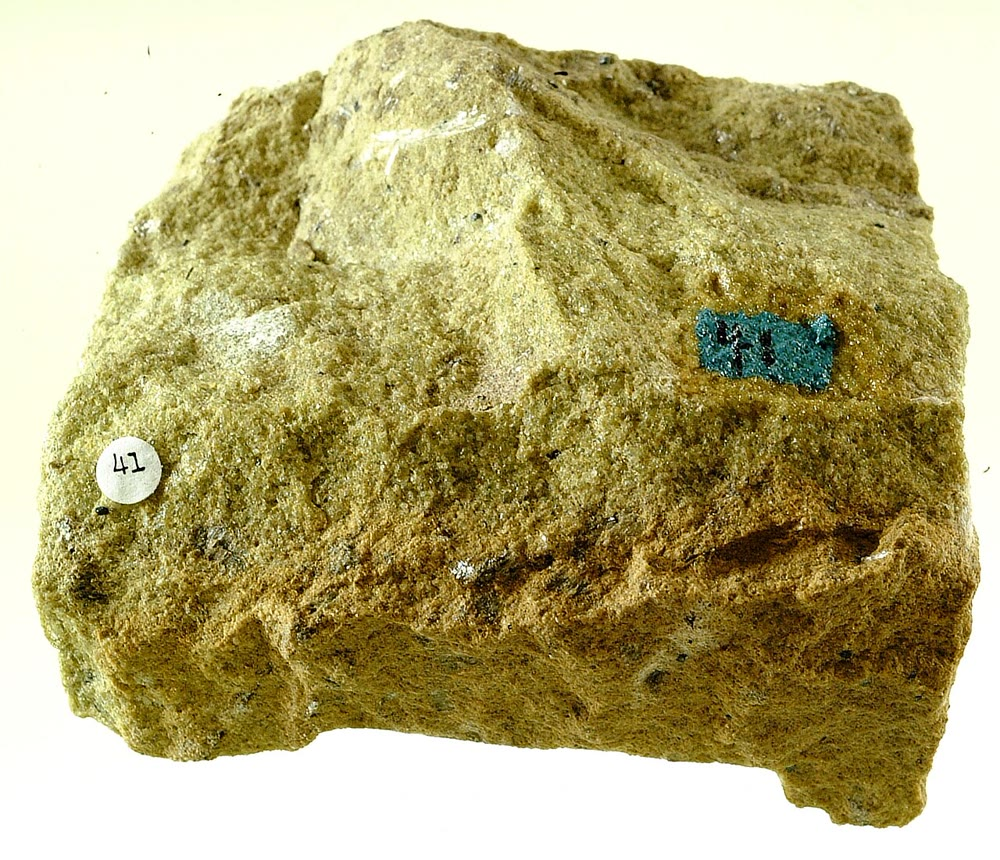
\includegraphics[width=\linewidth]{images/book4/b2-dunite.jpg}
\par\smallskip{\scriptsize Een \omterm{def:b2:mantle-melting:peridotites}{duniet}, bijna volledig olivijn, met kleine zwarte
korrels chromiet; het monster is \qty{8.5}{cm} breed (Mike Davis, CC0).}
\end{minipage}
\end{inthefield}
% ledger: casetta23:kimberlite, tulane:ocean-basins (Book 2), bgs:ultramafic

\section{Oefeningen}

\begin{exercise}[$\star$]\label{exo:b2:mantle-melting:1}
Benoem elk gesteente naar zijn verhoudingen van olivijn, orthopyroxeen en clinopyroxeen
(procent): (a) 93, 5, 2; (b) 75, 25, 0; (c) 60, 27, 13; (d) 30, 45, 25. (e) Geef
de naam van de model-bovenmantel (57, 28, 13 en \qty{2}{\percent} spinel) nadat
zijn drie silicaten tot \qty{100}{\percent} zijn hergenormaliseerd.
\end{exercise}
% ledger: bgs:ultramafic, liang21:dmm-mode

\begin{exercise}[$\star$]\label{exo:b2:mantle-melting:2}
Op het diagram diopsied--anorthiet koelt een smelt van \qty{60}{\percent} anorthiet
af. (a) Bij welke temperatuur begint hij te kristalliseren, en welk mineraal
vormt zich? (b) Bij welke temperatuur verschijnt het tweede mineraal, en wat is dan
de samenstelling van de smelt? (c) Wat is de samenstelling van de eerste smelt wanneer
een gesteente van \qty{80}{\percent} diopsied en \qty{20}{\percent} anorthiet wordt verhit,
en bij welke temperatuur verschijnt die?
\end{exercise}
% ledger: bowen15:di-an

\begin{exercise}[$\star$]\label{exo:b2:mantle-melting:3}
(a) Bereken de adiabatische gradiënt $\alpha T/(\rho c_p)$ in kelvin per gigapascal
voor $T_p = \qty{1350}{\celsius}$, $\alpha = \qty{4.0e-5}{K^{-1}}$, $\rho =
\qty{3300}{kg/m^3}$, $c_p = \qty{1000}{J/(kg.K)}$. (b) Hoeveel kilometer
mantel komt overeen met een gigapascal ($g = \qty{9.81}{m/s^2}$)? Reken de gradiënt om naar kelvin
per kilometer en vergelijk met een typische geothermische gradiënt dicht bij het oppervlak,
ongeveer \qty{30}{K/km}.
\end{exercise}
% ledger: katz03:thermo, earle:settings (Book 2)

\begin{exercise}[$\star$]\label{exo:b2:mantle-melting:4}
(a) Bereken de droge solidus van \omterm{def:b2:mantle-melting:peridotites}{peridotiet} bij 0, 1, 2 en \qty{3}{GPa}. (b) Met hoeveel
graden stijgt hij per gigapascal rond \qty{2}{GPa}? (c) Leg in één
zin uit waarom een mantel van \qty{1400}{\celsius} bij \qty{3}{GPa} vast is, en dezelfde
mantel, zonder warmte-uitwisseling naar \qty{2}{GPa} gebracht, gedeeltelijk gesmolten is.
\end{exercise}
% ledger: katz03:solidus

\begin{exercise}[$\star\star$]\label{exo:b2:mantle-melting:5}
Een smelt van \qty{70}{\percent} diopsied en \qty{30}{\percent} anorthiet koelt af.
(a) Schat zijn liquidustemperatuur door te interpoleren tussen de liquidus bij
\qty{20}{\percent} anorthiet (\qty{1350}{\celsius}) en bij \qty{40}{\percent}
(\qty{1277.5}{\celsius}). (b) Welk mineraal kristalliseert als eerste? (c) Welke
massafractie van het systeem is gekristalliseerd wanneer de smelt het eutecticum bereikt?
(d) Wat zijn de verhoudingen van diopsied en anorthiet in het uiteindelijke gesteente?
\end{exercise}
% ledger: bowen15:di-an

\begin{exercise}[$\star\star$]\label{exo:b2:mantle-melting:6}
(a) Bereken het massapercentage \ce{SiO2} in forsteriet \ce{Mg2SiO4} en in
enstatiet \ce{MgSiO3} ($M_{\ce{MgO}} = \qty{40.30}{g/mol}$, $M_{\ce{SiO2}} =
\qty{60.08}{g/mol}$). (b) Bowen en Andersen vonden dat de peritectische smelt
\qty{97.5}{\percent} \ce{MgSiO3} en \qty{2.5}{\percent} \ce{SiO2} bevat: wat is haar
silicagehalte? (c) Bereken met de hefboomregel de massafractie forsteriet
die ontstaat wanneer enstatiet in het \omterm{def:b2:mantle-melting:peritectic}{peritectisch punt} smelt, en vergelijk met hun
\qty{5.5}{\percent}. (d) Wat betekent dit voor het silicagehalte van een smelt van
\omterm{def:b2:mantle-melting:peridotites}{peridotiet} vergeleken met dat van zijn orthopyroxeen?
\end{exercise}
% ledger: bowen14:mgo-sio2

\begin{exercise}[$\star\star$]\label{exo:b2:mantle-melting:7}
Bereken met de adiabaat $T = T_p + 20P$ en de droge solidus uit de tekst de
druk en de diepte ($\qty{30.9}{km}$ per gigapascal) waarop het smelten begint
voor (a) $T_p = \qty{1300}{\celsius}$ en (b) $T_p = \qty{1450}{\celsius}$. (c) Met
hoeveel kilometer per \qty{10}{\celsius} verdiept het begin zich rond
$T_p = \qty{1300}{\celsius}$? Gebruik \cref{prop:b2:mantle-melting:onset}.
\end{exercise}
% ledger: katz03:solidus

\begin{exercise}[$\star\star$]\label{exo:b2:mantle-melting:8}
Neem bij \qty{2.0}{GPa} aan dat de \omterm{def:b2:mantle-melting:fraction}{smeltfractie} lineair stijgt van de droge solidus tot
de liquidus van \omterm{def:b2:mantle-melting:peridotites}{lherzoliet} $T_{\mathrm l} = 1475.0 + 80.0P - 3.2P^2$. Voor $F = 0.10$:
(a) bereken de temperatuur van het smeltende gesteente; (b) bereken $(\partial
T/\partial P)_F$ en $(\partial T/\partial F)_P$; (c) bereken de productiviteit met
$c_p = \qty{1000}{J/(kg.K)}$, $\alpha/\rho = \qty{1.21e-8}{m^3/(kg.K)}$ en
$\Delta S = \qty{300}{J/(kg.K)}$. (d) Hoeveel zou ze zijn zonder latente warmte?
\end{exercise}
% ledger: katz03:solidus, katz03:melting, katz03:thermo

\begin{exercise}[$\star\star$]\label{exo:b2:mantle-melting:9}
(a) Met hoeveel verlagen 1, 5 en \qty{13}{\percent} water opgelost in de smelt
de solidus? (b) Wat is de watergezadigde solidus bij \qty{1}{GPa}? (c) Een mantel
bevat \qty{125}{ppm} water in massa, en de verdelingscoëfficiënt van water tussen
mineralen en smelt is 0.01. Bij het allereerste smelten bevat de smelt $X =
X_{\text{totaal}}/D$: bereken die waarde en de verlaging van de solidus die ze veroorzaakt.
\end{exercise}
% ledger: katz03:water

\begin{exercise}[$\star\star\star$]\label{exo:b2:mantle-melting:10}
(a) Controleer in \cref{prop:b2:mantle-melting:triangle} dat de mantel die elk jaar de
basis van de driehoek binnenkomt, gelijk is aan de mantel die via zijn zijden vertrekt. Waarom
moeten de zijden onder \ang{45} staan voor een mantel die met $U$ opstijgt en met $U$ vertrekt?
(b) Toon aan dat bij constante productiviteit $\Pi$ per gigapascal $h_c = \Pi\,\rho
g\,z_0^2/2$ (met $P_0 = \rho g z_0$), zodat de korst groeit als het kwadraat van de
diepte van het begin. (c) Een rug spreidt met een volle snelheid van \qty{50}{mm/yr} en
maakt \qty{7.1}{km} korst: welk volume korst maakt elke kilometer rug
per jaar, en welk volume mantel smelt hij als de gemiddelde \omterm{def:b2:mantle-melting:fraction}{smeltfractie}
\qty{12}{\percent} is?
\end{exercise}

\begin{exercise}[$\star\star\star$]\label{exo:b2:mantle-melting:11}
In het ternaire systeem van de schematische figuur heeft de smelt $X$
\qty{60}{\percent} A, \qty{20}{\percent} B en \qty{20}{\percent} C; het
binaire eutecticum $e_{AB}$ ligt bij A 40, B 60 (procent), en het \omterm{def:b2:mantle-melting:ternary}{ternaire eutecticum} E bij
A 25, B 30, C 45. (a) Schrijf de samenstelling van de smelt wanneer een massafractie $t$
zuiver A is gekristalliseerd, en toon aan dat de verhouding van B tot C op 1 blijft. (b) De
\omterm{def:b2:mantle-melting:ternary}{cotectische lijn} van $e_{AB}$ naar E is de lijn van de punten $e_{AB} + s(E - e_{AB})$: zoek
waar de smelt haar ontmoet, en de fractie A die dan is gekristalliseerd. (c) Welke fractie van het systeem
is nog vloeibaar wanneer de smelt E bereikt? (C komt vóór E in geen enkel
kristal terecht.) (d) Hoeveel A en hoeveel B zijn er tegen dan gekristalliseerd?
\end{exercise}

\begin{exercise}[$\star\star\star$]\label{exo:b2:mantle-melting:12}
Het watergehalte van een verzadigde smelt is $X_{\mathrm{sat}} = 12P^{0.6} + P$
(procent, $P$ in gigapascal). (a) Bereken het bij 1 en \qty{2}{GPa}, de verlaging van de solidus
die het geeft, en de watergezadigde solidus bij beide drukken. (b) Waarom verandert
de verzadigde solidus nauwelijks tussen 1 en \qty{2}{GPa}, terwijl de droge
meer dan \qty{100}{\celsius} stijgt? (c) Hoeveel water moet de smelt in een mantelwig bij \qty{2}{GPa} en
\qty{1100}{\celsius} bevatten opdat het gesteente smelt?
\end{exercise}
% ledger: katz03:water, katz03:solidus

\section{Probleem: Onder de rug}

\begin{problem}[{Weekendprobleem --- van de manteladiabaat naar de dikte van
de oceanische korst, en terug naar de temperatuur van de mantel}]
\label{pb:b2:mantle-melting:1}
Mantel stijgt onder een rug op langs de adiabaat en smelt. Gegevens: thermische
uitzettingscoëfficiënt $\alpha = \qty{4.0e-5}{K^{-1}}$; dichtheid $\rho = \qty{3300}{kg/m^3}$;
soortelijke warmte $c_p = \qty{1000}{J/(kg.K)}$; smeltentropie $\Delta S =
\qty{300}{J/(kg.K)}$; $g = \qty{9.81}{m/s^2}$; droge solidus $T_{\mathrm s} =
1085.7 + 132.9P - 5.1P^2$ en liquidus van \omterm{def:b2:mantle-melting:peridotites}{lherzoliet} $T_{\mathrm l} = 1475.0 +
80.0P - 3.2P^2$ (\unit{\celsius}, $P$ in \unit{GPa}); gemiddelde productiviteit van het
gefitte smeltmodel, $\Pi = \qty{9}{\percent}$ per gigapascal; reactiecoëfficiënt van
clinopyroxeen dicht bij het oppervlak 0.50; waargenomen korst \qty[uncertainty-mode=separate]{7.1 \pm 0.8}{km}
bij normale ruggen en \qty{20}{km} boven de kern van de IJslandpluim. Neem voor mantel
en korst dezelfde dichtheid.

\noindent\textbf{Deel I --- Waar het smelten begint.}
\begin{enumerate}
\item Reken $T_p = \qty{1350}{\celsius}$ om naar kelvin.
\item Bereken de adiabatische gradiënt $\alpha T_p/(\rho c_p)$ in kelvin per
gigapascal, en rond hem af op het dichtstbijzijnde tiental.
\item Hoeveel kilometer mantel komt overeen met één gigapascal? Geef de gradiënt in
kelvin per kilometer.
\item Schrijf met de adiabaat $T = 1350 + 20P$ de vierkantsvergelijking voor de begindruk
$P_0$ op en los ze op.
\item Geef de diepte en de temperatuur waarop het smelten begint.
\item Controleer dat de solidus bij $P_0$ dezelfde temperatuur geeft.
\end{enumerate}

\noindent\textbf{Deel II --- Hoeveel smelt.}
\begin{enumerate}[resume]
\item Bereken bij \qty{1.5}{GPa} de solidus, de liquidus van \omterm{def:b2:mantle-melting:peridotites}{lherzoliet} en hun
verschil.
\item Geef, met een \omterm{def:b2:mantle-melting:fraction}{smeltfractie} die lineair tussen beide stijgt, de temperatuur van
het gesteente bij $F = 0.10$, in graden Celsius en in kelvin.
\item Bereken daar $(\partial T/\partial P)_F$ en $(\partial T/\partial F)_P$.
\item Bereken de productiviteit van \cref{prop:b2:mantle-melting:productivity}, in
procent per gigapascal.
\item Het gefitte model geeft gemiddeld $\Pi = \qty{9}{\percent}$ per gigapascal.
Waarom is dat lager? Welke \omterm{def:b2:mantle-melting:fraction}{smeltfractie} bereikt de mantel met $\Pi$ aan het
oppervlak ($F_{\max}$)?
\item De modelmantel bevat \qty{13}{\percent} clinopyroxeen. Bij welke
\omterm{def:b2:mantle-melting:fraction}{smeltfractie} raakt het dicht bij het oppervlak op? Is het residu onder de as een
\omterm{def:b2:mantle-melting:peridotites}{lherzoliet} of een \omterm{def:b2:mantle-melting:peridotites}{harzburgiet}?
\end{enumerate}

\noindent\textbf{Deel III --- De korst.}
\begin{enumerate}[resume]
\item Gebruik \cref{prop:b2:mantle-melting:triangle} met $H = z_0$ om de
dikte van de korst te berekenen.
\item Wat is de gemiddelde \omterm{def:b2:mantle-melting:fraction}{smeltfractie} van de samengevoegde smelt?
\item Vergelijk met de waargenomen dikte.
\item Het volledige model van de figuur geeft \qty{9.0}{km}. Waarom is dat dunner dan
de schatting hierboven?
\item Toon aan dat $h_c = k P_0^2$ en bereken $k$ in kilometer per vierkante
gigapascal.
\end{enumerate}

\noindent\textbf{Deel IV --- De temperatuur van de mantel.}
\begin{enumerate}[resume]
\item Bereken de begindruk $P_0$ die \qty{7.1}{km} korst maakt.
\item Geef de overeenkomstige diepte van het begin.
\item Bereken met de adiabaat $T = T_p + 20P$ de potentiële temperatuur die
het begin bij die druk legt.
\item Herhaal de berekening voor 6.3 en \qty{7.9}{km}: welk bereik van $T_p$ laat de
spreiding van de korst toe?
\item De korst is \qty{20}{km} dik boven de kern van de IJslandpluim. Bereken
de potentiële temperatuur daar, en het overschot ervan boven die van vraag~20.
\item Lava's van oceaaneilanden wijzen op pluimen die 200 tot \qty{300}{\celsius} heter zijn dan
de omringende mantel. Geef een reden waarom de korst een kleiner overschot geeft.
\item Met hoeveel procent wordt de korst dikker voor een mantel die \qty{10}{\celsius}
heter is, dicht bij de normale rug?
\item Zeer trage ruggen maken dunnere korst. Verklaar dit met de driehoek.
\item Geef de potentiële temperatuur van de mantel onder een normale rug die
de dikte van de korst oplevert, het kerngetal van dit probleem, en vergelijk
ze met de \qty{1350}{\celsius} uit de mineraalfysica en het bereik 1280 tot
\qty{1400}{\celsius} uit lava's.
\end{enumerate}
\end{problem}
% ledger: katz03:solidus, katz03:melting, katz03:thermo, white:crust (Book 3), herzberg:tp (Book 3), katsura:adiabat (Book 3)
